\documentclass[a4paper,10pt]{article}

\usepackage[utf8]{inputenc}             % Input encoding
\usepackage[T1]{fontenc}                % Font encoding
\usepackage[english]{babel}             % English language features
\usepackage[yyyymmdd]{datetime}         % Reformatting dates
\usepackage[margin=1.5cm]{geometry}     % Margin tweaking
\usepackage{graphicx}                   % Images (maybe not necessary)
\usepackage{hyperref}                   % Hyper links
\usepackage[super]{nth}                 % Ordinals with exponent
\usepackage{enumitem}                   % List tools
\usepackage{wrapfig}

\setlist{noitemsep}                     % No huge separation between list points
\renewcommand{\dateseparator}{--}       % Change the date separator to --
\hypersetup{                            % Colors of URLS
    colorlinks=true,    
    urlcolor=blue,
}

\title{
    \textbf{Milestone 2: Team Data Viz' le 6}
}
\author{
    Beuchat Bastien \hspace{2cm} Jollès Eric \hspace{2cm} Robin Mamie
}

% MILESTONE 2 OBJECTIVES
% 1 Two A4 pages describing the project goal.
%
% 2  -  Include sketches of the vizualiation you want to make in your final product.
% 3  -  List the tools that you will use for each visualization and which (past or future) lectures you will need.
% 4  -  Break down your goal into independent pieces to implement. Try to design a core visualization (minimal viable product) that will be required at the end.
%
% 5 Then list extra ideas (more creative or challenging) that will enhance the visualization but could be dropped without endangering the meaning of the project.
%
% 6 Functional project prototype review.
%
% 7   -  You should have an initial website running with the basic skeleton of the visualization/widgets.

% 1 -
%   R - à voir à la fin
% 2 -
%   R - Bastien, aka Super Man, s'occupe de ça
% 3 -
%   R - TODO chiant mais faut faire pour chaque feature
% 4 -
%   R - Outline dans ce rapport, à relire et compléter
% 5 -
%   R - J'en ai mis quelques une, à rajouter
% 6 -
%   R - Est-ce que c'est nous qui devons le review, en disant ce qui est déjà bien et ce qu'il y a encore à faire ?
% 7 -
%   R - Bastien s'en occupe

\begin{document}

\maketitle

\section*{Introduction}

Our goal is to provide an easy way of visualizing the results of the FIS alpine skiing world cup's (WC) history, from 1966 to 2020.
The final interface presents itself as a control panel, where each one of our features will be present on the same web page.

\section{Core features}

Our main focus is to explore the results in time and space.
Since our dataset covers all the results from 1966 until 2020, it is indeed useful to be able to specify the \textit{current date} (it will designate the season) of the visualization.
This \textit{current date} will act as a conductor for all our features.

\subsection{Main timeline}

This first feature is not really a visualization but a very important tool to browse through the years.
It will define which season is used to compute the current displayed visualizations.

\subsection{Personal info page}

All skiers will have a personal information page, containing their name, birth date, profile picture, etc.
This page can be loaded by selecting a skier in any other visualization, i.e. the graph similarity, and the bar chart race or normal race rankings.
The quantity of personal information will depend on what is available online on the official FIS website.
There will also be different visualizations for each skier available into three different modes, either showing:

\begin{itemize}
\item Their whole career
\item Their career until the \textit{current date}
\item Their results of the season taking place on the \textit{current date}
\end{itemize}

These visualizations will be composed of:

\begin{itemize}
\item A global point tally, counting all the world cup points collected by the skier.
\item Specialized point tallies, counting all the WC points collected by the skier during specific events (slalom, downhill, etc.)
\item Their different rankings during their WC seasons.
These will be computed using the data we gathered, so they \textit{might} be different from the official rankings.
Indeed, it could be possible that points had been deducted outside of the races.
\item Their $n$ (probably 3 or 5) previous results in any given event.
\end{itemize}

A search feature allowing to search for a particular athlete will be provided.

\subsection{Ranking evolution}

In order to show the evolution of the general classification rankings in any given WC season, we decided to use bar chart race.
We based our graph on  \href{https://bl.ocks.org/jrzief/70f1f8a5d066a286da3a1e699823470f}{this visualization}. 
We added a slider to be able to move between race results.
We also added images for each skier, we will choose whether the profile picture or the image of their country's flag is most suitable.
We will attribute a color for each skier depending on their event specialty.
We will also add more bar chart races for every race specialty; they will be available in different tabs.

\subsection{Event map}

A map of the world will show all the events of any given season.
The top results of the events will be shown as a popover when clicking on them, and further race details will be shown in another panel.
The map will be linked to the rankings.
It will be animated alongside the bar-chart race, i.e. the map will show the event currently updating the rankings.

\subsection{Similarity graph}

A "similarity" graph shows the links between skiers, i.e. which skiers compete together in similar events.
A graph corresponds to the "topology" of a particular season.
This shows which skiers are completely specialized (e.g. only do slalom) and which are truly versatile.
Being able to browse through the seasons and compare evolution of the topology can really be very interesting and give a lot of information for ski fans.

Each node of the graph corresponds to a skier and a link is added between two skiers if they raced against each other at least K times during the season.
K is a threshold allowing us to drop less relevant links.
K has to be adapted through the years because there are far more races and skiers in 2020 compared to the first seasons.
The nodes will be clickable and can load skier information in the profile page.
We can use colors to highlight important node, for example the winner of a final ranking of the season.

\section{Tools}

\begin{description}
    \item[\href{https://d3js.org/}{D3.js} --] library used to draw our main visualizations (ranking evolution, similarity graph, personal info page).
    \item[\href{https://github.com/johnwalley/d3-simple-slider}{d3-simple-slider} --] used to have a slider element
    \item[\href{https://github.com/IonDen/ion.rangeSlider}{Ion.RangeSlider } --] not used currently, but we plan to build the timeline on it
    \item[\href{https://leafletjs.com/}{Leaflet} --] library used to display the map
    \item[\href{https://getbootstrap.com/}{Bootstrap} --] used for the layout of the whole website and some standard UI components (for example : buttons, tooltips, tabs)
    \item[\href{https://jquery.com/}{jQuery} --] dependency of Bootstrap and used directly for DOM manipulation and linking all the parts together.
    \item[\href{https://popper.js.org/}{Popper} --] dependency of Bootstrap
\end{description}

We are basing our work on the following lectures: \textit{Maps}, \textit{Interactions}, \textit{d3.js}.

\section{Extra visualizations and ideas}

For the personal info page, we could develop a simple metric showing who are the skier's main rivals.
This would be determined by e.g. the number of shared podiums, or contenders that have a similar number of WC points for a given discipline.

The times of different events of the same races could be compared in another visualization, as to compare whether races that keep their track more or less the same through history become faster or slower over time.

We can use the similarity graph to tell more characteristics of one season by extracting some graph properties.

Another cool extension is to adapt the dashboard to a fully mobile compatible version either with responsive design or a dedicated mobile web page. 

A feature of comparison between skiers could be provided.
This could be useful to get a sense on what type of skier is dominant during each season, if for example one chooses to compare 2 world cup winners of different seasons.
Their respective careers could be compared using a timeline showing the number of points each one of the skier gained at each age, during which events, etc.
We could also compare the results of the same skier during 2 different seasons.

\section{Prototype review}

\href{https://com-480-project-data-viz-le-6.github.io/}{Our prototype} already offers the basic visualizations described in this report.
Some features are obviously not yet implemented, but everything is at least drafted on it.
We will need to polish the UI and the layout and also link each component together.

\begin{center}
    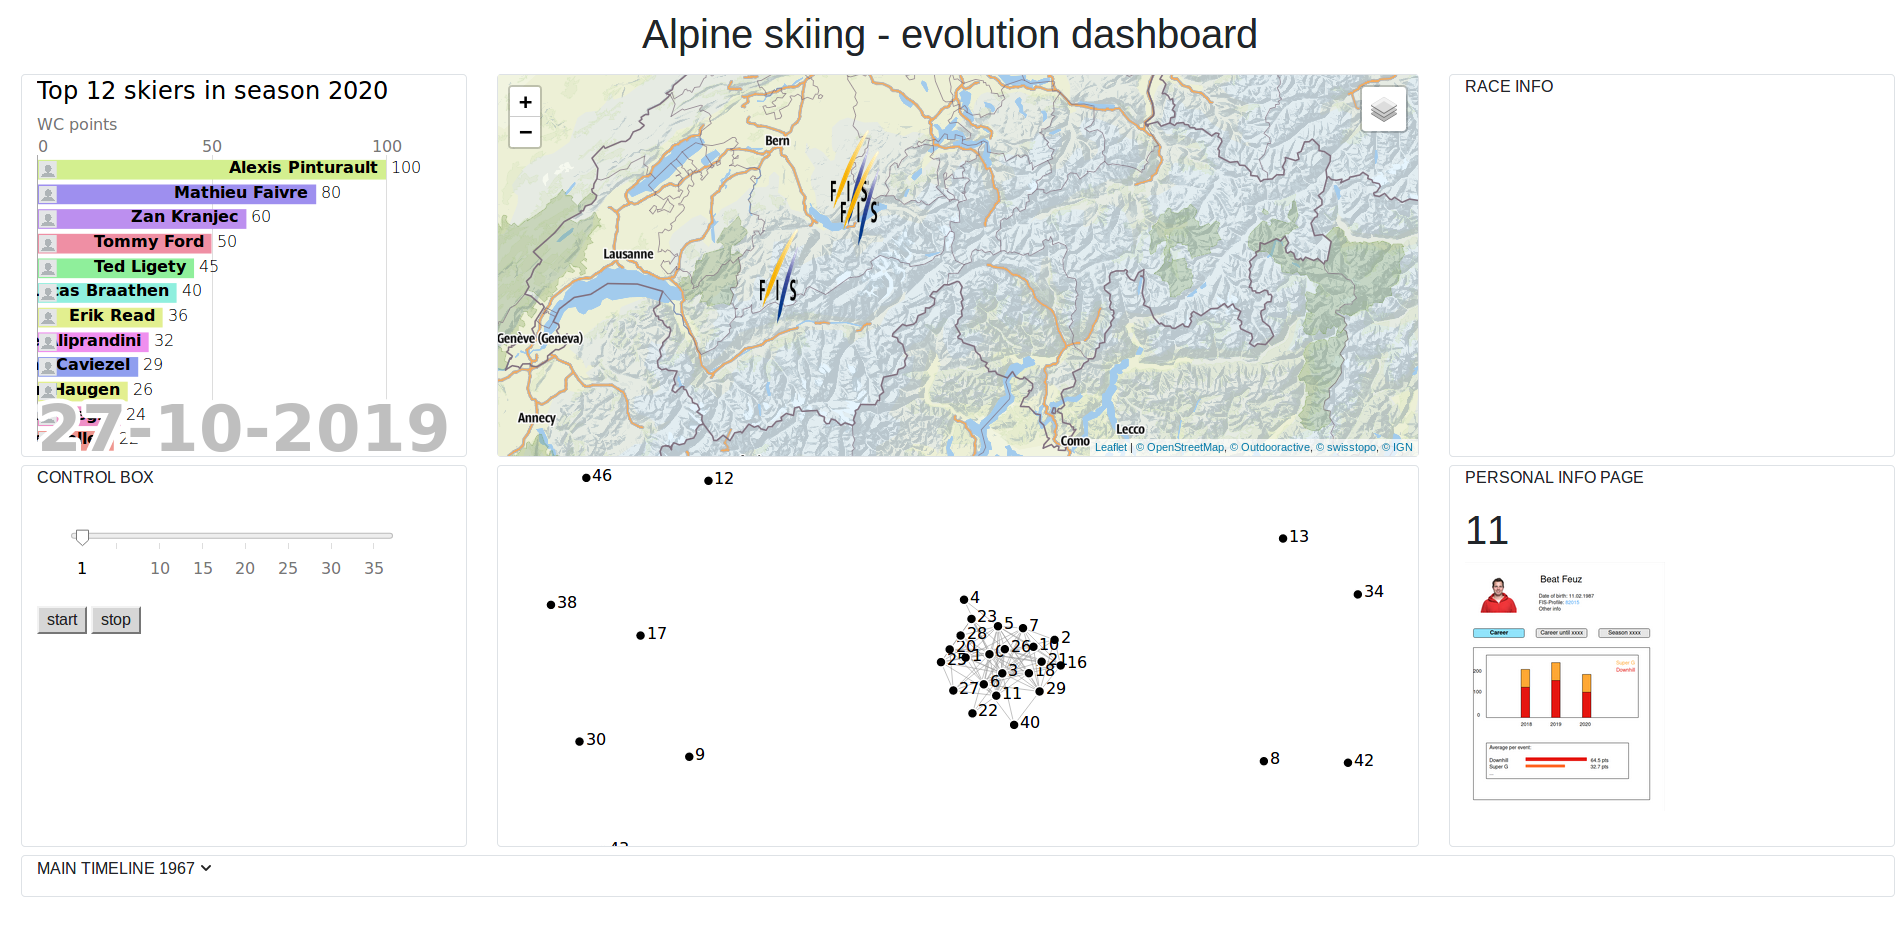
\includegraphics[width=0.8\textwidth]{prototype.png}
\end{center}

\end{document}
